%
% main.tex -- Paper zum Thema <thema>
%
% (c) 2018 Nicolas Tobler, Hochschule Rapperswil
%

\chapter{Klima auf anderen Planeten\label{chapter:thema}}
\lhead{Klima auf anderen Planeten}
\begin{refsection}
\chapterauthor{Nicolas Tobler}

\section{Einleitung}
\rhead{Einleitung}

\begin{figure}
	% https://www.astrobio.net/news-exclusive/comparing-climates-from-earth-to-exoplanets/
	\centering
	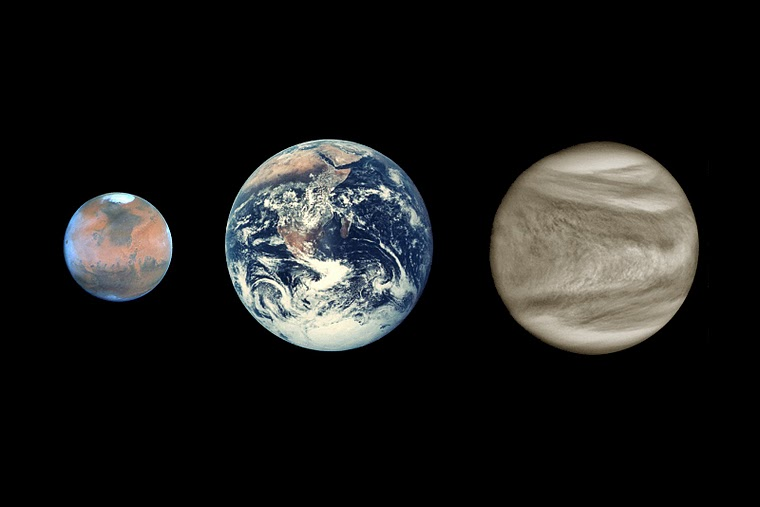
\includegraphics[width=0.7\linewidth, trim={0 3cm 0 3cm},clip]{planeten/Pictures/planets.jpg}
	\caption{Mars, Erde und Venus massstabsgerecht}
\end{figure}



%Verschiedene Organisationen, wie unter anderem Elon Musk's SpaceX, haben sich zum Ziel gemacht, in absehbarer Zukunft den Mars für den Menschen bewohnbar zu machen. Insbesondere sollte der Mars eine erdählnliche Atmosphere erhalte, also terraformed werden. Was auf Computer-generierten bildern ziemlich simpel aussieht, wird sich in realität wahrscheinlich ziemlich schwierig herausstellen. In diesem Kapitel wird die aktuelle lage des Klimas auf dem Mars analysiert und mögliche Wege den Mars zu teraformen auf die Machbarkeit untersucht.



venus co2 bindung
wie ist venus co geworden


was führt zu wasserlosen athmosphere
mars keine
venus ohne wasser
erde zwischendrin

boxmodell anteile element


%Grinspoon said, “It may be that conditions for life’s origin aren’t rare, but the hard part is the persistence of habitable conditions.”

Auf allen Planeten kann flüssiges Wasser auftreten (Godilooks-Zone).

\begin{center}
\begin{table}
	\center
	\begin{tabular}{l|c c c c}
                      & Mars    & Erde   & Venus           & Merkur\\
  \hline
  Temperatur (Mittel) & 218 K   & 288 K  & 737 K           & 440 K\\
  Wolken              & $<5\%$ & $68\%$ & $\approx100\%$ & - \\
  Atmosphäre          & $6 \cdot 10^{-3}$ bar & $1$ bar & $92$ bar & $10^{-15}$ bar
	%\hline
	
\end{tabular}
\caption{Planeten im Vergleich}
\end{table}

\end{center}

Merkur ist in der Tabelle vertreten um zu verdeutlichen, dass nahe an der Sonne nicht direkt eine heisse Mitteltemperatur bedeutet.


\subsection{Temperatur}

\subsection{Albedo}

\subsection{Atmosphereische Eigenschaften}

dünne Atmosphere

Wann und wieso verlor der Mars seine Atmosphäre


Rückgang der Atmosphäre durch Sonnenwind
	https://www.nasa.gov/press-release/nasa-mission-reveals-speed-of-solar-wind-stripping-martian-atmosphere


\subsection{Treibhausgase}

wasser

co2


\section{Modell}
\rhead{Modell}


	Für alle Planeten geltendes Modell erstellen
	
	Das Modell sollte Erdähnliche Bedingungen bewusst erstreben, um zu sehen ob diese auf den Planeten Mars und Venus auch bestehen können.
	
	Betrachtet wird ein früher Zeitpunkt der Geschichte des Sonnensystems, als die betrachteten Planeten ähnliche oder annähernd gleiche materielle und Atmosphärische Eigenschaften aufwiesen.
	
	Es wird vor allem angenommen, dass grosse Mengen an Wasser auf allen Planeten vorhanden war.
	
%	Desshalb wird 
	
	Andere klimabestimmenden atmosphärischen Gase werden nicht simuliert, um das Modell im gegebenen Rahmen umzusetzen.
	%Um das Modell im beschränkem Zeitrahmen zu realisieren, kann nur ein hoch vereinfachtes Modell erstellt werden.

	
	Vereinfacht: Erde nehmen, auf Mars Grösse skallieren, in den Mars-Orbit setzten und schauen was passiert. 
	

Das hier erarbeitete Modell konzentriert sich nur auf die Strahlungsbillanz und den Wasserkreislauf.

%Wasser wurde gewählt, da auf allen Planeten flüssiges Wasser auftreten kann (Godilooks-Zone).
Wasser stellt auf der Erde den grössten Anteil zum Treibhauseffekt bei.
Des Weiteren ist es für den Menschen interessant Planeten mit Erdähnlichen Zuständen anzutreffen.



 Dazu müssen einige Annahmen getroffen werden.	
	
	Annahmen
		Gleiche materielle Eigenschaften
		Gleiches Vorkommen an Wasser
		Wasser hat grösste Auswirkung auf Klima
	
	
Möglichst auf einfachen Physikalischen Gesetzen basieren.	
	
	
Am Schluss müssen freie Parameter abgeschätzt werden, um überhaubt plausible Lösungen zu erreichen.


\begin{figure}
	\centering
	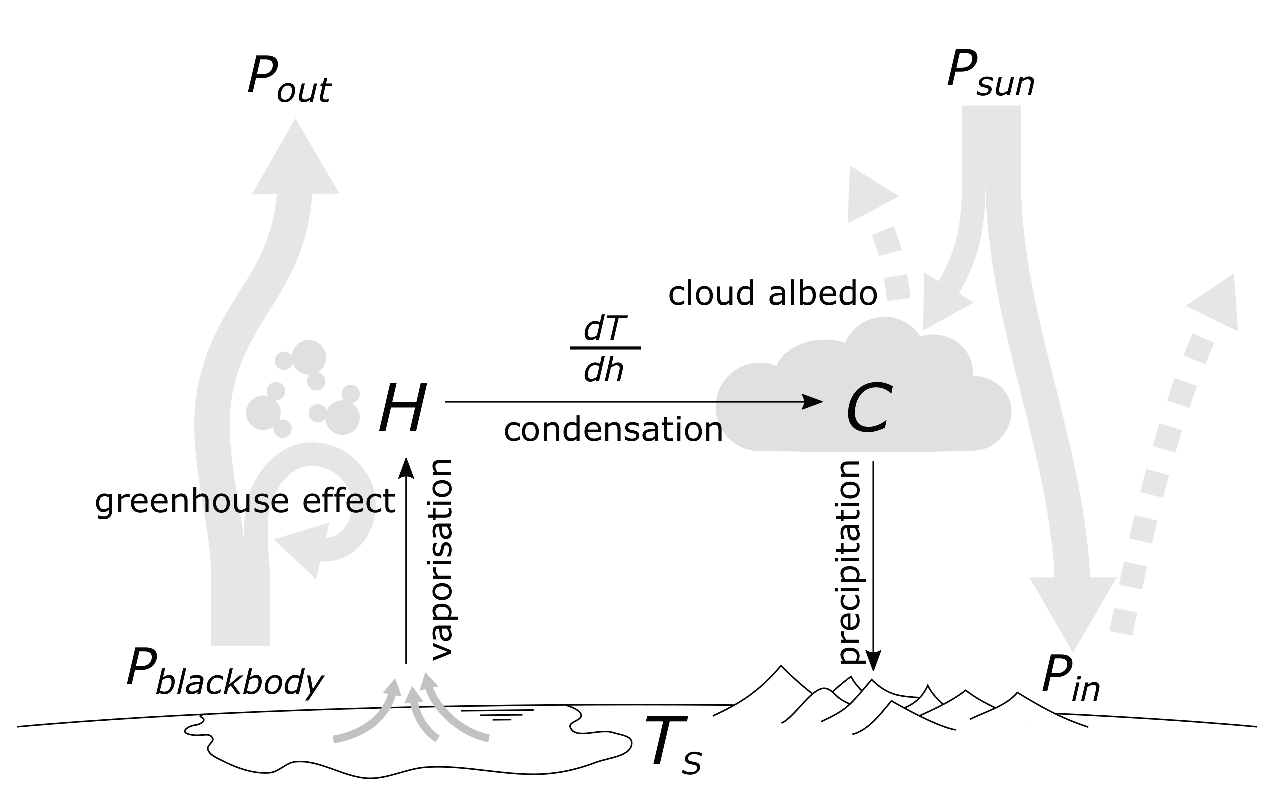
\includegraphics[width=\textwidth]{planeten/Pictures/Model.eps}
	\caption{Modell}
\end{figure}

\subsection{Strahlungsbilanz}

Die Strahlungsbillanz wird in Kapitel \hl{reference needed} ausführlich beschrieben. Das hier verwendeten Modell baut direkt darauf auf.

Damit die Durchschnittstemperatur eines Planeten stabil ist, muss die Leistungsbilanz Null sein.

\begin{equation}
\dot{T} = \xi_1(P_{in} - P_{out})
\end{equation}

Die Eintreffende Leistung $P_{in}$ besteht primär aus der absorbierten Sonnenstrahlung. Andere Energiequellen wie ein Aktives Planet-Inneres und die Energie aus Gezeiten wird vernachlässigt. Es gilt:

\begin{equation}
P_{in} = \sigma T_{\astrosun}^4 \left( \frac{R_{\astrosun}}{a_{planet}} \right) ^2 \cdot (1-\alpha)
\end{equation}

Dabei ist $\alpha$ das Albedo des Planeten.

Die Abgestrahlte Leistung besteht praktisch ausschliesslich aus der Black-body strahlung, welche sich aus der Durchschnittstemperatur $T$ und dem Radius $R$ des Planeten bestimmen lässt. Diese Leistung bleibt jedoch teilweise durch Treibhausgase in der Atmosphäre gefangen. Es gilt: 

\begin{equation}
P_{out} = (4 \pi R^2 \sigma T_{S}^4)\epsilon
\end{equation}

Dabei ist $\sigma$ die Stefan-Boltzmann-Konstante und $\epsilon$ der Anteil der durchdringenden Leistung.

\subsection{Albedo}

Das Albedo wird als Funktion der prozentualen Wolkenabdeckung $C$ modelliert. Es wird ein linearer Zusammenhang erwartet.

\begin{equation}
\alpha(C) = (0.65 \cdot C) + 0.15;
\end{equation}


Unter der Annahme, dass bei allen Planeten das Oberflächenalbedo $\alpha_{surface}$ gleich ist, wird ein minimales $\alpha_{min}$ und maximales Albedo $\alpha_{max}$ definiert. Bei 100\% Wolkendeckung soll der Maximalwert erreicht werden und bei 0\% das Oberflächenalbedo.

\begin{equation}
\alpha = \alpha_{surface} + C(\alpha_{max} - \alpha_{surface})
\end{equation}

\subsection{Treibhauseffekt}

Wasserdampf ist ein sehr effektifes Treibhausgas. Es wird angenommen dass der atmosphärische Wasserdampf der Erde für 60\% des Treibhauseffekts sorgt.  

% 60\%    % https://www.acs.org/content/acs/en/climatescience/climatesciencenarratives/its-water-vapor-not-the-co2.html 

Im verwendeten Modell wird diese linear zum Teibhauseffekt $\beta$ modelliert.

\begin{equation}
\epsilon  = (1 - \beta) = (1 - 0.5 \cdot H)
\end{equation}

\subsection{Wasserkreislauf}

Modellierung von atmosphärischem Wasserdampf $H$ als relative Luftfeuchtigkeit und Wolken $C$ als prozentuale Flächendeckung.


\subsubsection{Wasserdampfbildung}

Linearer Zusammenhang zur Auftreffenden Leistung

\begin{equation}
\xi_4 (P_{in})
\end{equation}

\subsubsection{Wolkenbildung}

\begin{equation}
\xi_5 H \frac{dT}{dh}
\end{equation}

Der Temperaturgradient wird linear Angenommen somit lässt sich $\frac{dT}{dh}$ durch $\Delta T $ vereinfachen. 

\begin{equation}
\xi_5 H \Delta T
\end{equation}

\subsubsection{Wolkenabbau}

linear zur Wolkenabdeckung

\begin{equation}
\xi_6 C
\end{equation}

\subsection{Zusammengefasst}

\begin{equation}
	\begin{matrix}			
		\dot{H} = & \xi_4 P_{in}(C) & - \xi_5 H \Delta T & \\
		\dot{C} = &                 &   \xi_5 H \Delta T & - \xi_6 C
	\end{matrix}	
\end{equation}


%\subsection{Entweichen von atmosphärischen Gasen}
%
%Ob ein Planet oder Mond eine Atmosphäre besitzt ist von wenigen parametern abhängig. Planeten behalten ihr Atmosphäre, wenn die Gravitation ausreichend stark ist, um die Moleküle gegen ihre thermische Geschwindigkeit zurückzuhalten.
%Die Moleküle in der Atmosphäre, für die
%
%% https://www.tcd.ie/Physics/people/Peter.Gallagher/lectures/PY4A03/pdfs/PY4A03_lecture12n13_amospheres.ppt.pdf
%
%\begin{equation}
%v_{escape} > v_{therm}
%\end{equation}
%
%zutrifft, werden nach und nach in den Weltraum abgestossen.
%Die Fluchtgeschwindigkeit eines Planeten $v_{escape}$ wird durch deren Masse $M$ und Radius $R$ berechnet: 
%
%\begin{equation}
%v_{escape} = \sqrt{\frac{2GM}{R}}
%\end{equation}
%
%wobei $G$ die Gravitationskonstante ist. Die Fluchtgeschwindigkeit ist somit bei grossen und schweeren Gestirnen grösser.
%
%Die thermische Geschwindigkeit eines Moleküls ist Maxwell-Bolzmann-verteilt. Deshalb gilt der berechnete Wert in diesem Zusammenhang nur approximativ. Die höchst wahrscheinliche Geschwindigkeit ist: 
%
%\begin{equation}
%v_{therm} = \sqrt{\frac{3kT}{m}}
%\end{equation}
%
%Dabei ist $k$ die Bolzmann-Konstante und $m$ die Mol-Masse des Moleküls. Die kritische Temperatur $T_{escape}$, bei welcher Gase abgestossen werden ist somit:
%
%\begin{equation}
%T_{escape} = \frac{2GMm}{3kR}
%\end{equation}

\subsection{Differentialgleichung}

\begin{equation}
\left|
\begin{matrix}
\dot{T} = &  & \xi_1 \left(P_{in}(C) - P_{out}(T, H) \right) &\\
\dot{H} = & \xi_4 P_{in}(C) & - \xi_5 H \Delta T & \\
\dot{C} = &                 &   \xi_5 H \Delta T & - \xi_6 C
\end{matrix}
\right|
\end{equation}

Um zu verhindern, dass eine Luftfeuchtigkeit oder Wolkenabdeckung von über 100\% auftritt, werden zu gewissen linearen Termen noch den gleichen Term mit grosser Potenz dazu addiert. Somit wird der Effekt verstärkt wenn die Grösse nahe an $1$ also $100\%$ kommt.  

Mit Anpassungen für gesättigten Wasserdampf und Wolkenabdeckung:

\begin{equation}
\left|
\begin{matrix}
\dot{T} = & & \xi_1 \left(P_{in}(C) - P_{out}(T, H) \right) &\\
\dot{H} = & \xi_4 P_{in}(C) & - \xi_5 (H + H^9) \Delta T & \\
\dot{C} = &                 &   \xi_5 (H + H^9) \Delta T & - \xi_6 (C + C^5)
\end{matrix}
\right|
\end{equation}


\section{Simulation}
\rhead{Simulation}

Das Modell wurde in MATLAB mittels Transientenanalyse simuliert. Dazu wurde ein ode45 Solver benutzt.




Die Anfangswerte wurden so gesetzt, dass sie Erd-Bedinugnen unterstützen  
	Erdbedingungen
	
	System anregen Erdähnliche Werte zu generieren.

\begin{equation}
\begin{matrix}
T_0 = & 283 \\
H_0 = & 0.5 \\
C_0 = & 0.5
\end{matrix}
\end{equation}

\subsection{Ergebnisse}

		Die Strich-Punkt-Linie der entsprechenden Farbe zeigt den heutigen Wert der Grösse. 

		\begin{figure}
			\center
			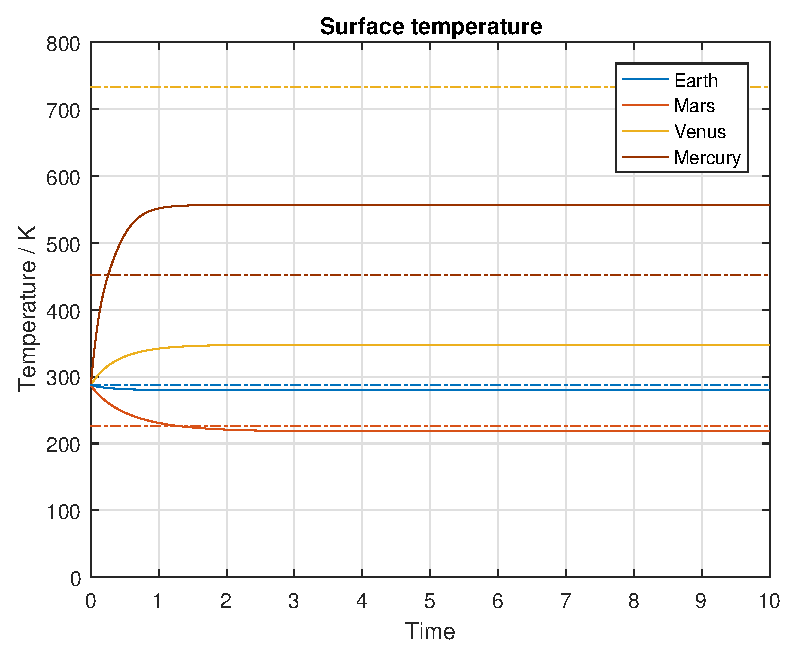
\includegraphics[height=0.45\textheight]{planeten/Matlab/figures/surfaceTemperature.eps}
			\caption{Globale Durchschnittstemperatur}
		\end{figure}
		
		\begin{figure}
			\center
			\includegraphics[height=0.45\textheight]{planeten/Matlab/figures/humidity.eps}
			\caption{Relative Luftfeuchtigkeit}
		\end{figure}
		
		\begin{figure}
			\center
			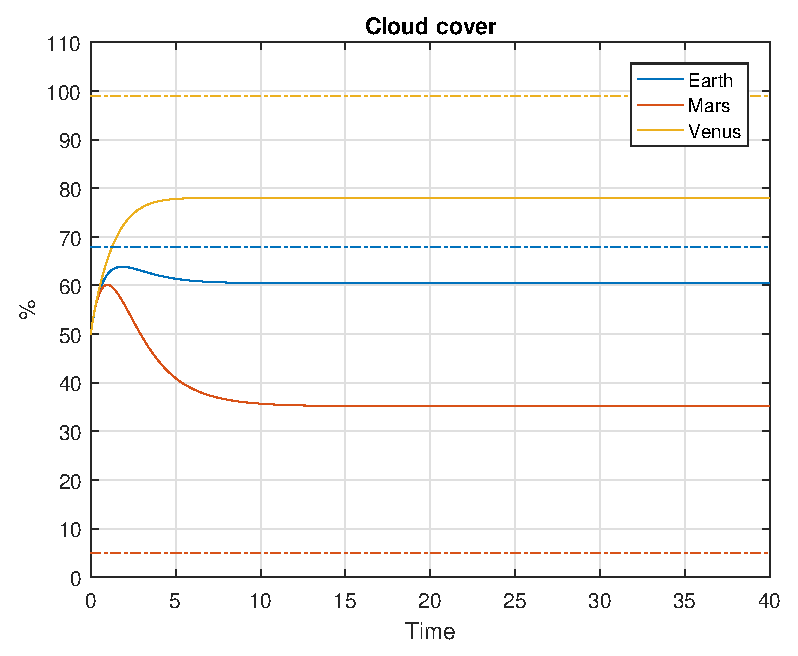
\includegraphics[height=0.45\textheight]{planeten/Matlab/figures/cloudCover.eps}
			\caption{Prozentuale Wolkenabdeckung}
		\end{figure}
		
		\begin{figure}
			\center
			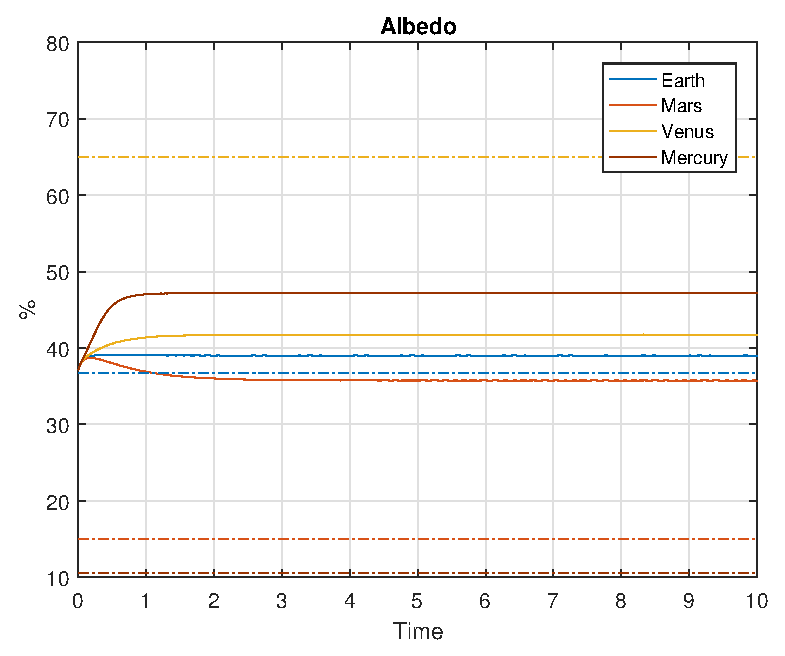
\includegraphics[height=0.45\textheight]{planeten/Matlab/figures/albedo.eps}
			\caption{Albedo}
		\end{figure}

\section{Schlussfolgerung}
\rhead{Schlussfolgerung}

Ergebnisse gleichen dem heutigen Status
Extremes Klima von Mars \& Venus vermutlich prädestiniert

Abweichungen

Ergebnisse nur mit Vorsicht zu geniessen

Nicht modelierte faktoren:
Nur Wasser simuliert
Chemische und Physikalische Vorgänge bei extremen Temperaturen

Andere Treibhausgase wie CO$_2$, welches heute den grössten Anteil der Venus- und Marsatmosphäre ausmacht, vernachlässigt.

\subsection{Verbesserungsmöglichkeiten}

Nächste Schritte das Modell zu verbessern

Um mehr Genauigkeit in den Extremen Bereichen zu erreichen, müssten mehr atmosphärische Gase einbezogen werden.
Diese Gase besitzen wiederum unterschiedliche Gefrierpunkte, was die Modellierung der Vereisung zulässt.
		
Im simulierten Modell wurden lediglich der Durchmesser und die Distanz zur Sonne der Planeten einbezogen. Um die Aussagekraft zu verbessern könnten weitere Planet-abhängige Parameter implementiert werden, wie der Vulkanismus und die Rotationsgeschwindigkeit. Die Rotation erlaubt das Modellieren von Tag- und Nachtseitentemperatur, welche sich stark auf das Klima auswirken.


\printbibliography[heading=subbibliography]
\end{refsection}
